\subsection{Experimental Setup}
\label{sec:exp_protocol}

\noindent\textbf{Hardware, tasks, and data collection.}
The evaluation includes $5$ single-arm and $4$ bimanual tasks on the two platforms shown in Fig.~\ref{fig:robot_setup}; the tasks are summarized in Fig.~\ref{fig:task_overview}. The single-arm platform is a 7-DoF Franka Emika Panda with wrist-mounted and external Intel RealSense D405 cameras. Demonstrations are collected using a 3Dconnexion SpaceMouse. The bimanual platform is an X Square Robot with one wrist-mounted camera per arm and one shared external camera. Demonstrations are collected through leader--follower teleoperation. Following ForceVLA~\cite{yu2025forcevlaenhancingvlamodels}, both platforms use robot-provided joint-torque-based wrench estimates without additional wrist force/torque sensors.

For each task, we collect $200$ demonstrations. Multi-view images, robot states, and commanded actions are recorded at $30$~Hz, and timestamped wrench estimates at $100$~Hz.

\begin{figure}[t]
    \centering
    \begin{minipage}[c]{0.45\columnwidth}
        \centering
        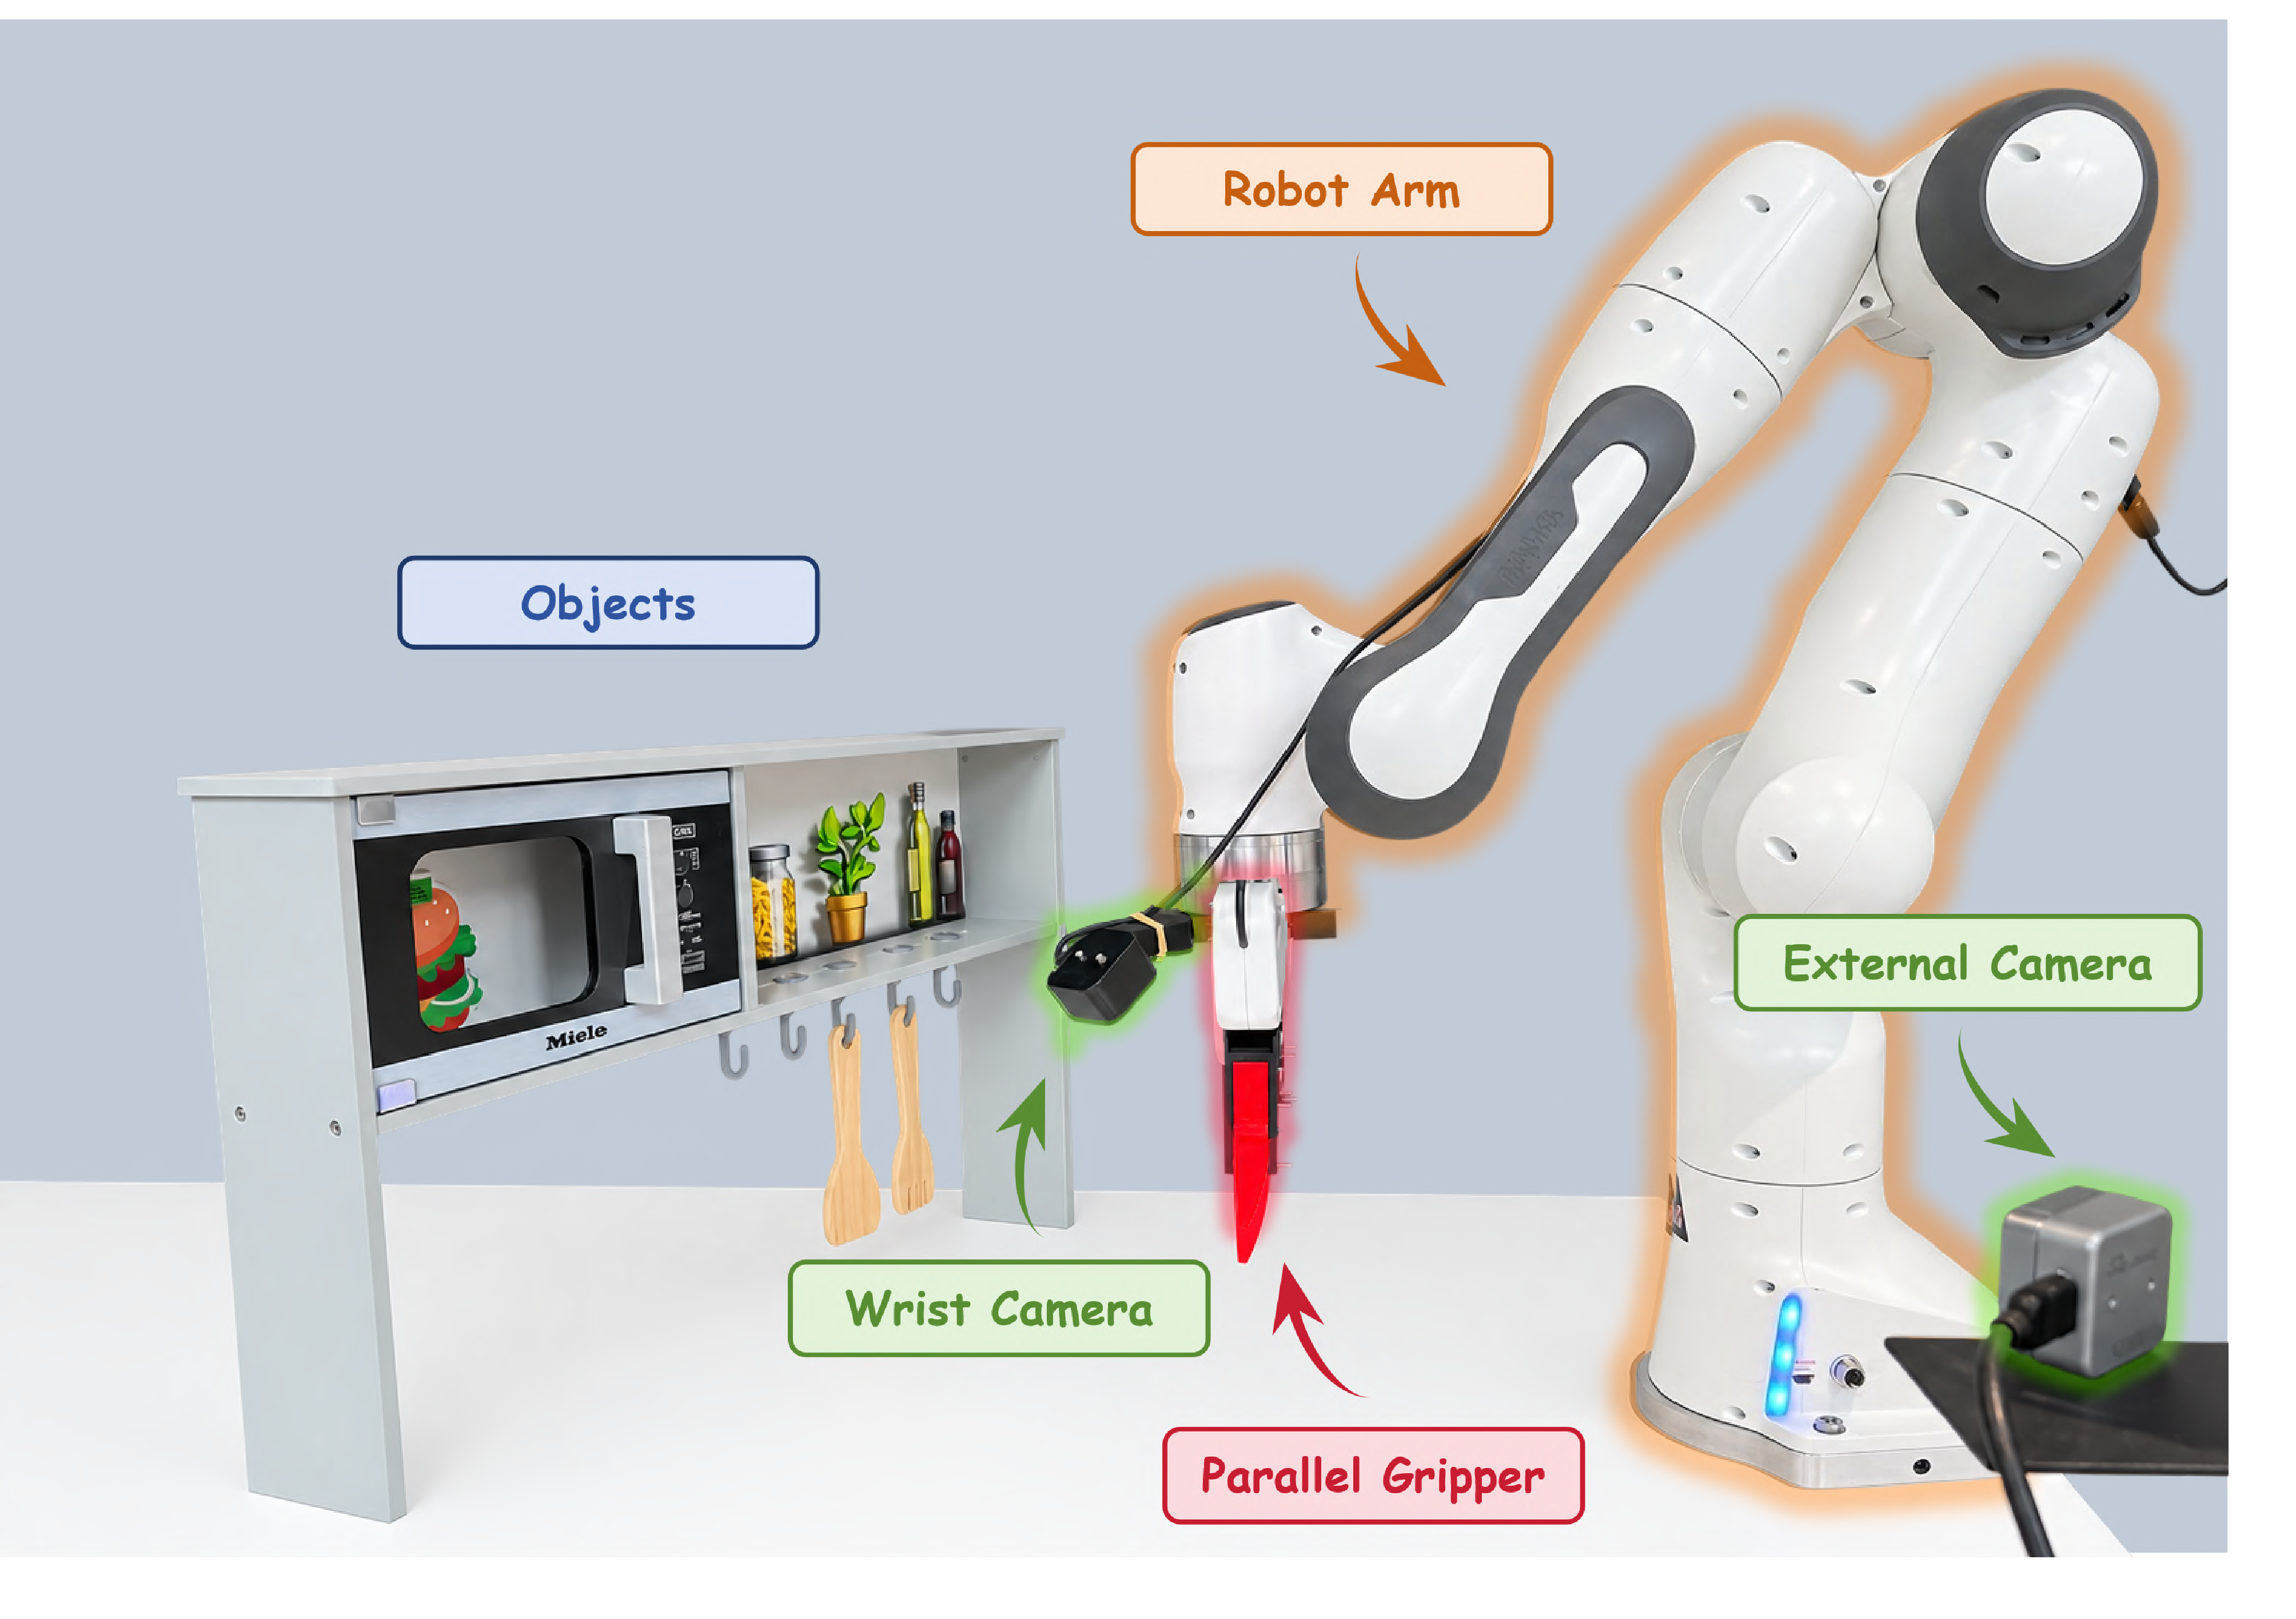
\includegraphics[width=\linewidth]{figures/fig04a_franka_platform.pdf}
    \end{minipage}\hspace{0.025\columnwidth}
    \begin{minipage}[c]{0.45\columnwidth}
        \centering
        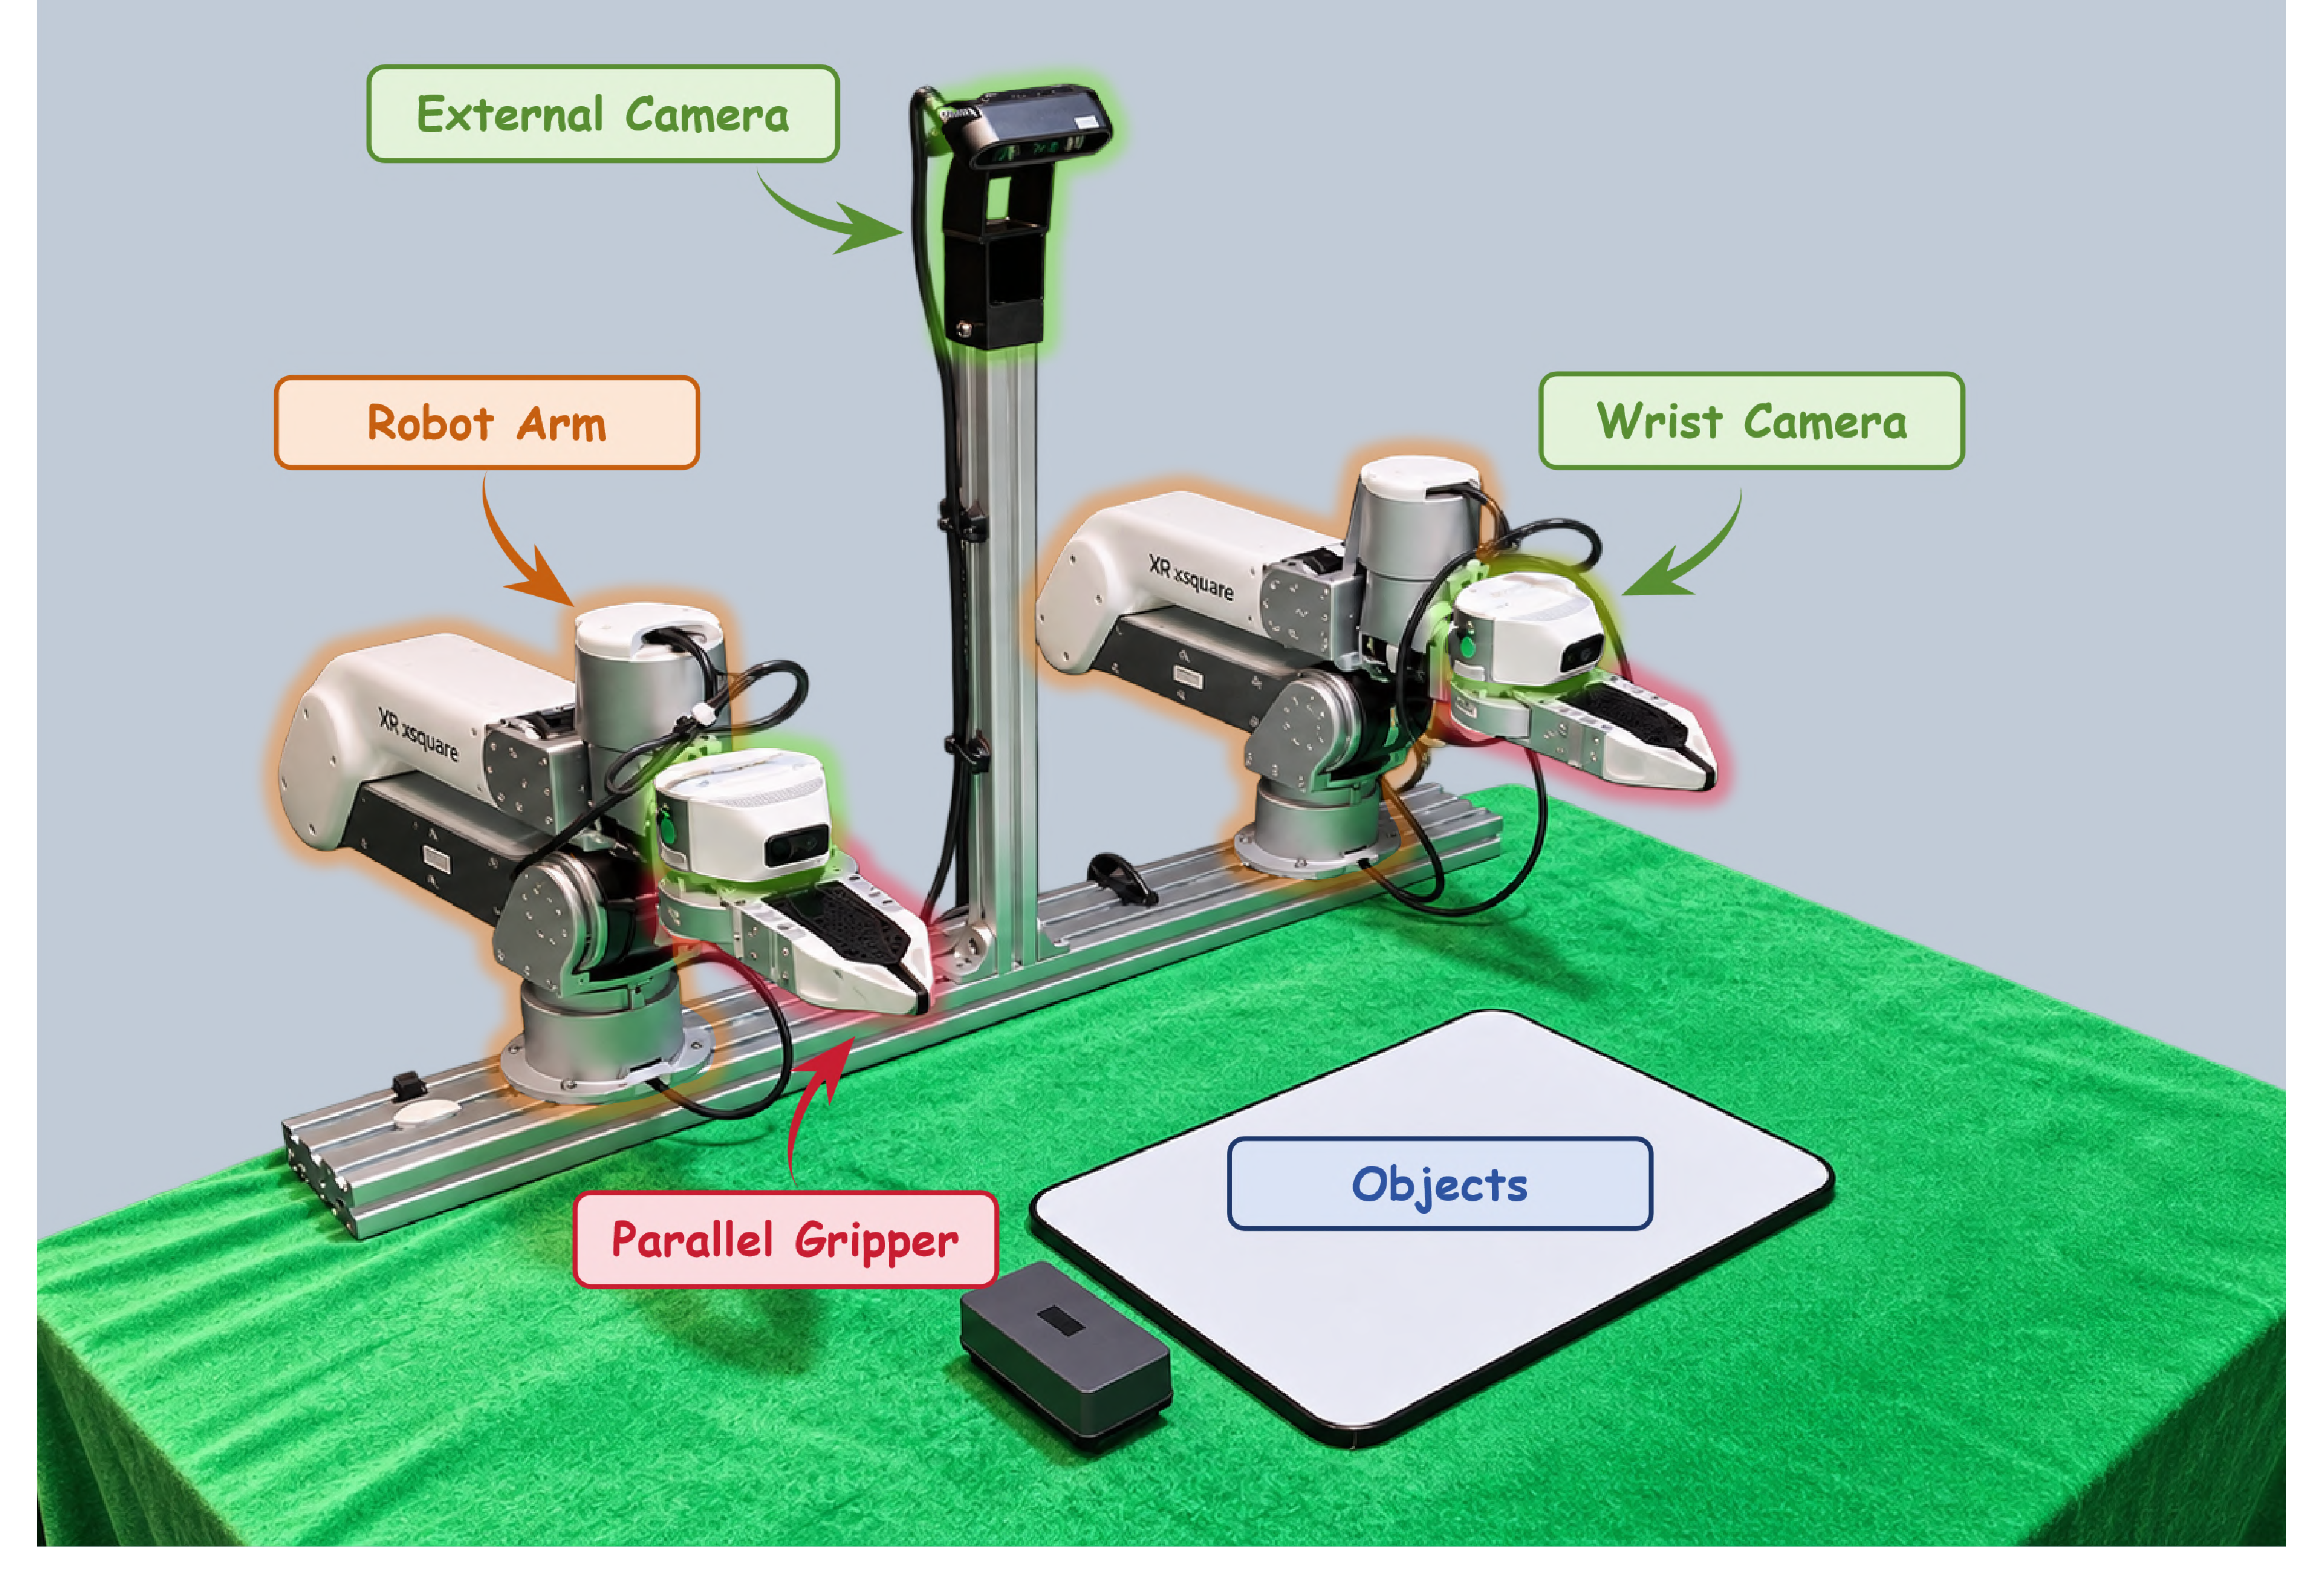
\includegraphics[width=\linewidth]{figures/fig04b_bimanual_platform.pdf}
    \end{minipage}
    \caption{Real-robot platforms. Left: single-arm Franka. Right: bimanual X Square Robot.}
    \label{fig:robot_setup}
\end{figure}

\begin{figure}[t]
    \centering
    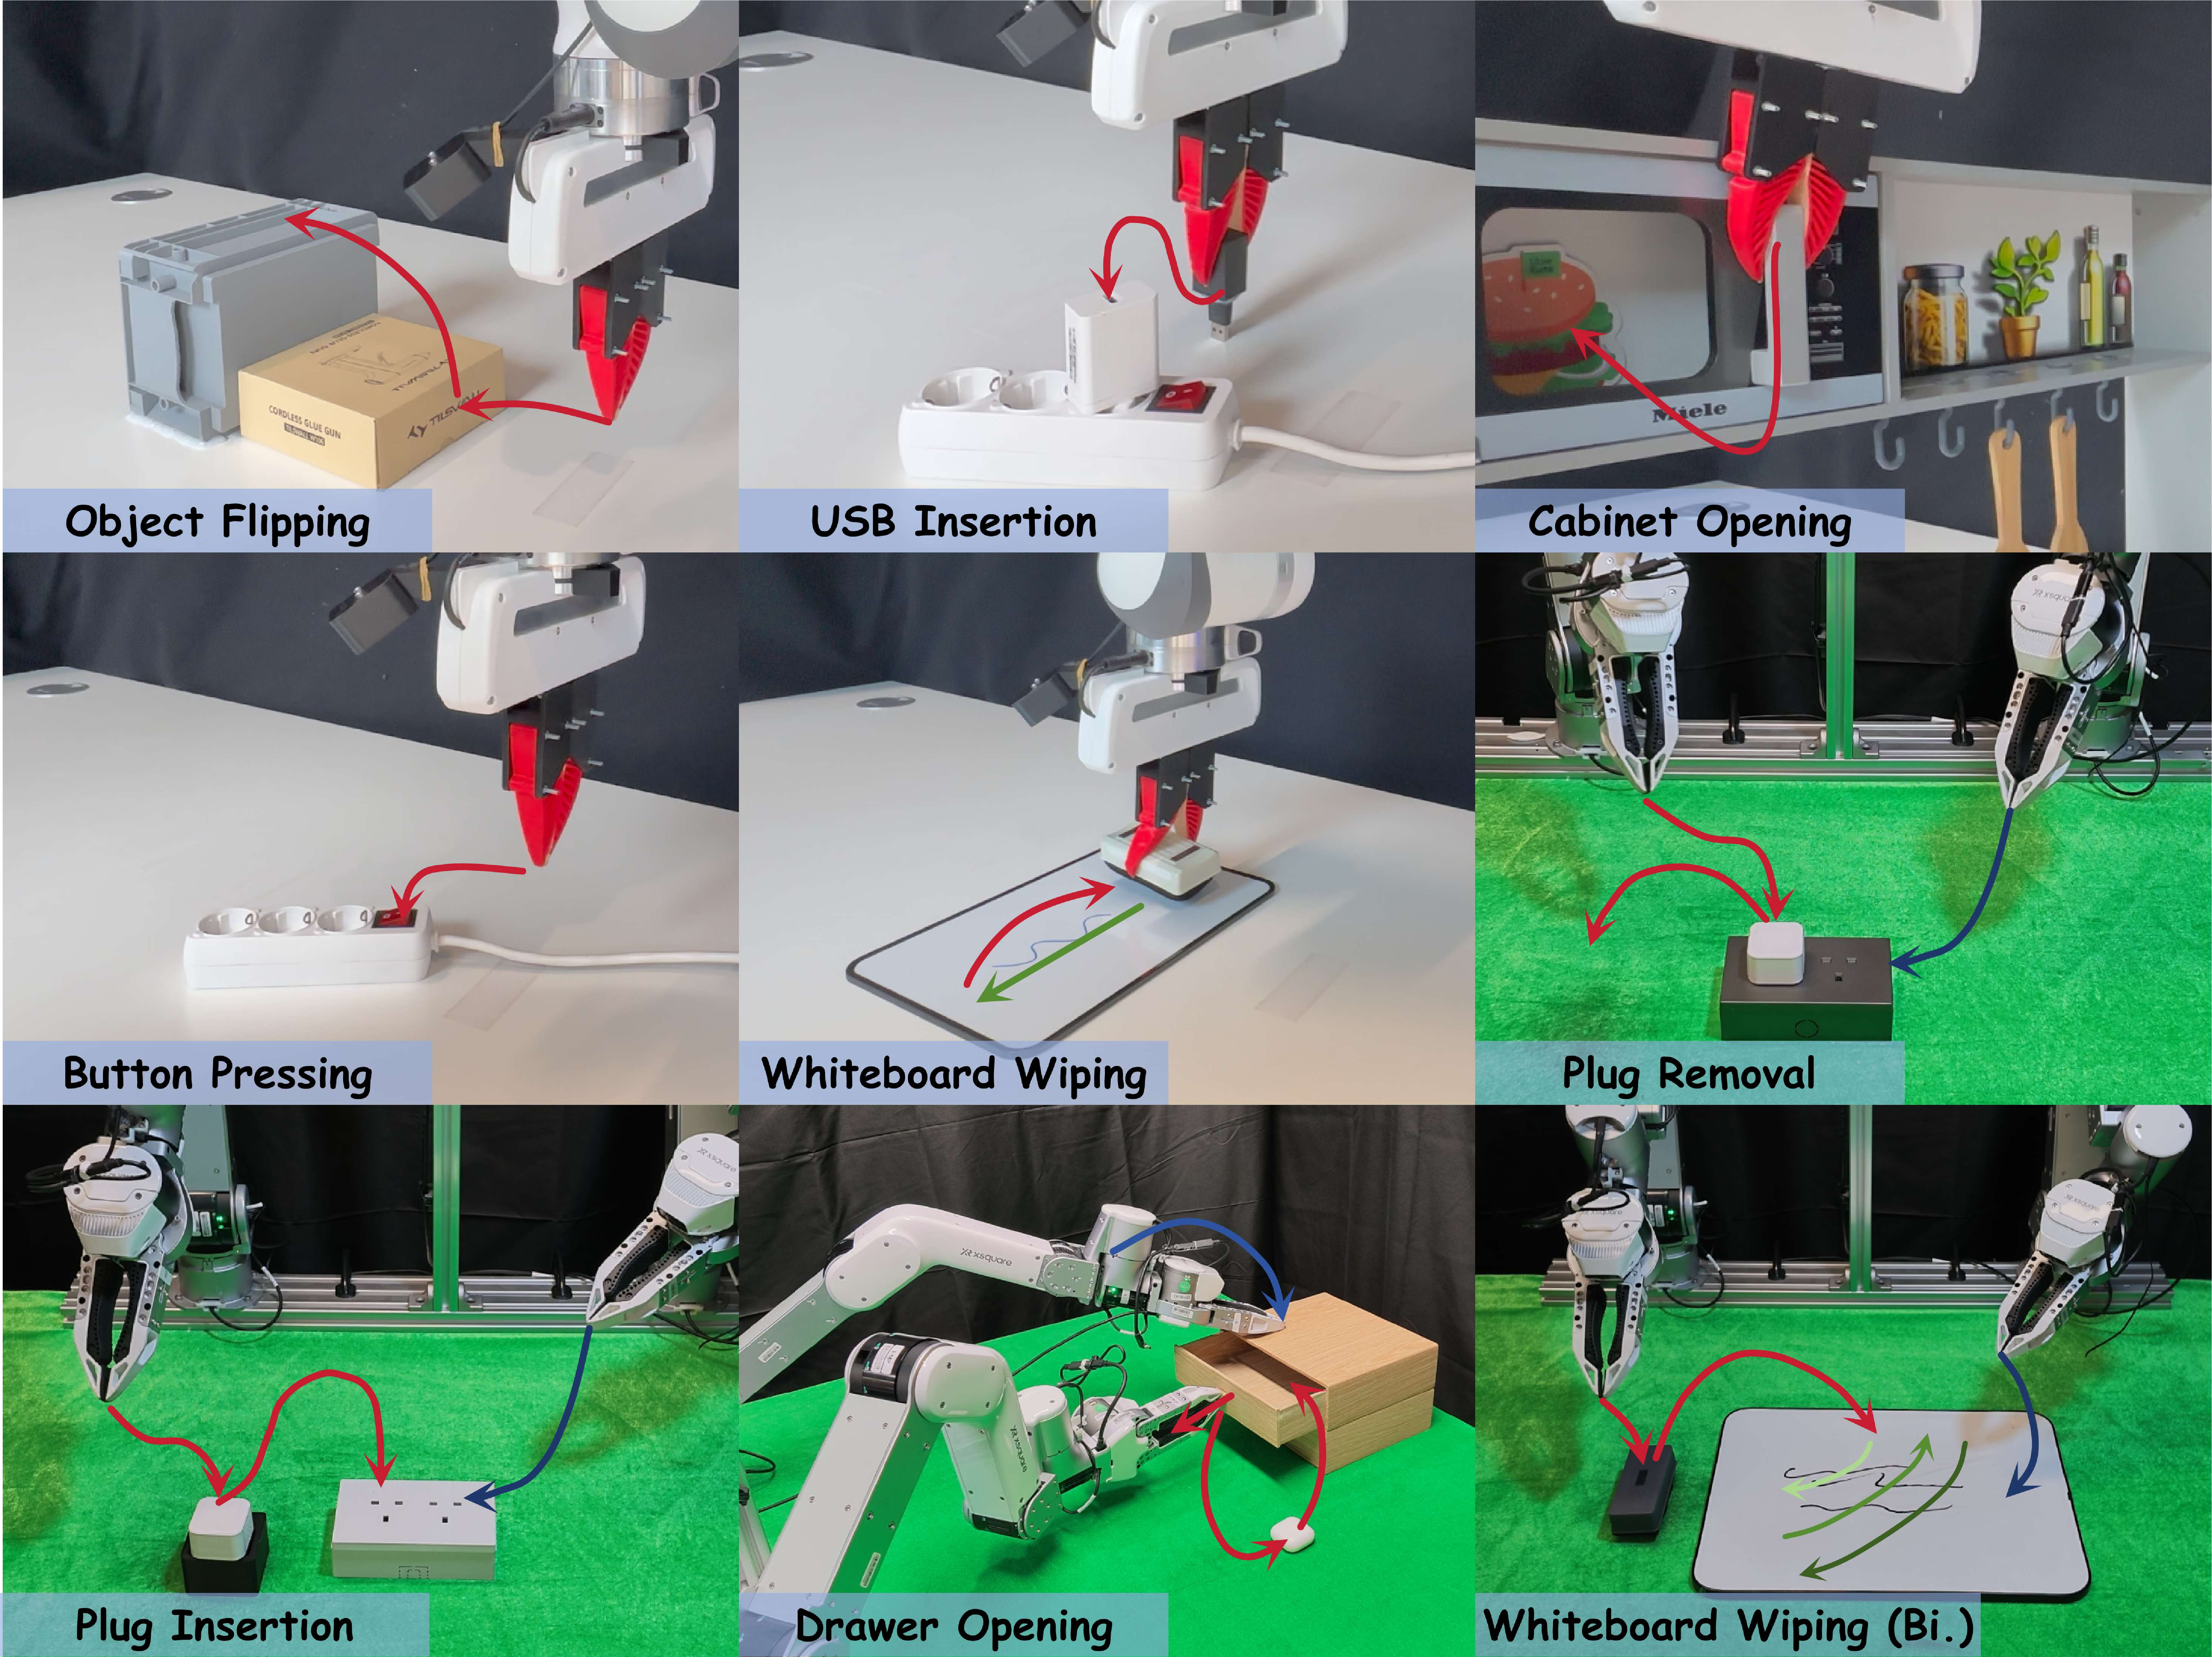
\includegraphics[width=\columnwidth]{figures/fig05_task_overview.pdf}
    \caption{The nine real-robot manipulation tasks used in the evaluation. The first five panels show single-arm tasks; the remaining four show bimanual tasks.}
    \label{fig:task_overview}
\end{figure}

\begin{table*}[!t]
    \centering
    \scriptsize
    \setlength{\tabcolsep}{3pt}
    \caption{Task success rate (\%) over 20 trials per method and task; Avg. is the mean across the nine tasks.}
    \label{tab:main_results}
    \begin{tabular}{lcccccccccc}
        \toprule
        & \multicolumn{5}{c}{\textbf{Single-arm}} & \multicolumn{4}{c}{\textbf{Bimanual}} & \\
        \cmidrule(lr){2-6}\cmidrule(lr){7-10}
        \textbf{Method}
        & \shortstack{Object\\Flipping}
        & \shortstack{USB\\Insertion}
        & \shortstack{Cabinet\\Opening}
        & \shortstack{Button\\Pressing}
        & \shortstack{Whiteboard\\Wiping}
        & \shortstack{Plug\\Removal}
        & \shortstack{Plug\\Insertion}
        & \shortstack{Drawer\\Opening}
        & \shortstack{Whiteboard\\Wiping}
        & \textbf{Avg.} \\
        \midrule
        $\pi_{0.5}$~\cite{intelligence2025pi05visionlanguageactionmodelopenworld} & 55.0 & 35.0 & 50.0 & 45.0 & 70.0 & 40.0 & 30.0 & 50.0 & 50.0 & 47.2 \\
        ForceVLA~\cite{yu2025forcevlaenhancingvlamodels} & 65.0 & 40.0 & 60.0 & 50.0 & 70.0 & 50.0 & 35.0 & 60.0 & 60.0 & 54.4 \\
        TA-VLA~\cite{zhang2025tavlaelucidatingdesignspace} & 65.0 & 35.0 & 60.0 & 60.0 & 75.0 & 55.0 & 40.0 & 60.0 & 65.0 & 57.2 \\
        ImplicitRDP~\cite{chen2026implicitrdpendtoendvisualforcediffusion} & 50.0 & 25.0 & 45.0 & 35.0 & 65.0 & 55.0 & 30.0 & 55.0 & 45.0 & 45.0 \\
        Temporal Teacher & 75.0 & 55.0 & 75.0 & 80.0 & 85.0 & 75.0 & 50.0 & 70.0 & 70.0 & 70.6 \\
        \textbf{ForceDelta-VLA (Ours)} & \textbf{90.0} & \textbf{80.0} & \textbf{80.0} & \textbf{85.0} & \textbf{90.0} & \textbf{80.0} & \textbf{70.0} & \textbf{80.0} & \textbf{85.0} & \textbf{82.2} \\
        \bottomrule
    \end{tabular}
\end{table*}

\noindent\textbf{Baselines and evaluation protocol.}
We compare with ForceVLA~\cite{yu2025forcevlaenhancingvlamodels}, a force-aware full-action policy that also provides our teacher backbone; $\pi_{0.5}$~\cite{intelligence2025pi05visionlanguageactionmodelopenworld}, a VLA without force/torque input; TA-VLA~\cite{zhang2025tavlaelucidatingdesignspace}, a torque-aware VLA; and ImplicitRDP~\cite{chen2026implicitrdpendtoendvisualforcediffusion}, a slow--fast visual--force policy. We also evaluate direct execution of the Stage-1 Temporal Teacher used by ForceDelta-VLA. All methods use the same task demonstrations, initial-state distributions, controller settings, and safety limits. We report success rate, peak contact force, and completion time.

\noindent\textbf{Implementation details.}
The teacher encodes a $100$-ms wrench history and predicts an action chunk with $H{=}50$ steps. The correction policy uses a causal force encoder and a shared attention module with separate force- and delay-correction heads to predict $K{=}5$ pose corrections. Deployment runs on a workstation with two NVIDIA RTX 4090 GPUs. The reference-action forward pass averages $189.7$~ms, corresponding to approximately $5$~Hz for serial inference (Table~\ref{tab:runtime}). Robot command transmission is limited to $100$~Hz; this control rate is distinct from the correction-query rate. Training and optimization details are provided in the supplementary material.

\subsection{Main Results}
\label{sec:exp_main}

\noindent\textbf{Quantitative results.}
Compared with the original ForceVLA baseline, the complete ForceDelta-VLA system improves mean success from $54.4\%$ to $82.2\%$ (Table~\ref{tab:main_results}). It also exceeds TA-VLA, $\pi_{0.5}$, and ImplicitRDP. Success improves over ForceVLA on all nine tasks, with the largest gains on USB Insertion, Button Pressing, and Plug Insertion.

Direct execution of the Stage-1 Temporal Teacher achieves $70.6\%$ mean success. ForceDelta-VLA improves mean success by about $11.7$ percentage points over this teacher. The largest gains are on USB Insertion and Plug Insertion, at $25$ and $20$ points, respectively. On Button Pressing, most of the improvement over ForceVLA is already obtained by the Temporal Teacher ($50\%$ to $80\%$); ForceDelta-VLA raises success to $85\%$.

\noindent\textbf{Contact force and completion time.}
Relative to ForceVLA, mean peak contact force over successful trials decreases by $4.2$~N on the single-arm platform and $4.3$~N on the bimanual platform, approximately $26\%$ on each (Table~\ref{tab:interaction}). Mean completion time decreases by $5.2$~s and $5.9$~s, respectively. Relative to the Temporal Teacher, the peak-force reductions are $3.3$~N and $2.2$~N, and completion time decreases by $3.9$~s and $3.4$~s.

\begin{table}[t]
    \centering
    \scriptsize
    \setlength{\tabcolsep}{2pt}
    \caption{Peak force and completion time, reported as mean $\pm$ standard deviation over successful trials pooled across tasks within each platform.}
    \label{tab:interaction}
    \begin{tabular}{lcccc}
        \toprule
        & \multicolumn{2}{c}{\textbf{Peak force} (N) $\downarrow$} & \multicolumn{2}{c}{\textbf{Completion time} (s) $\downarrow$} \\
        \cmidrule(lr){2-3}\cmidrule(lr){4-5}
        \textbf{Method} & Single & Biman. & Single & Biman. \\
        \midrule
        $\pi_{0.5}$ & $18.9 \pm 8.3$ & $20.4 \pm 9.1$ & $30.4 \pm 11.2$ & $33.1 \pm 12.8$ \\
        ForceVLA & $16.0 \pm 4.7$ & $16.8 \pm 6.2$ & $29.1 \pm 6.5$ & $31.7 \pm 9.4$ \\
        TA-VLA & $16.5 \pm 6.4$ & $15.9 \pm 4.8$ & $28.2 \pm 9.7$ & $30.0 \pm 7.1$ \\
        ImplicitRDP & $15.2 \pm 5.1$ & $14.8 \pm 4.9$ & $27.1 \pm 7.2$ & $27.4 \pm 7.8$ \\
        Temporal Teacher & $15.1 \pm 5.8$ & $14.7 \pm 4.3$ & $27.8 \pm 8.8$ & $29.2 \pm 6.9$ \\
        \textbf{\shortstack[l]{ForceDelta-VLA\\(Ours)}} & $\mathbf{11.8} \pm 3.4$ & $\mathbf{12.5} \pm 2.9$ & $\mathbf{23.9} \pm 5.4$ & $\mathbf{25.8} \pm 7.6$ \\
        \bottomrule
    \end{tabular}
\end{table}

\noindent\textbf{Qualitative results.}
Figure~\ref{fig:qualitative_button} highlights how the learned translational correction evolves through contact. The correction is smaller before sustained contact, increases during pressing, shows a brief change near peak contact, and decreases as contact is released.

\begin{figure}[t]
    \centering
    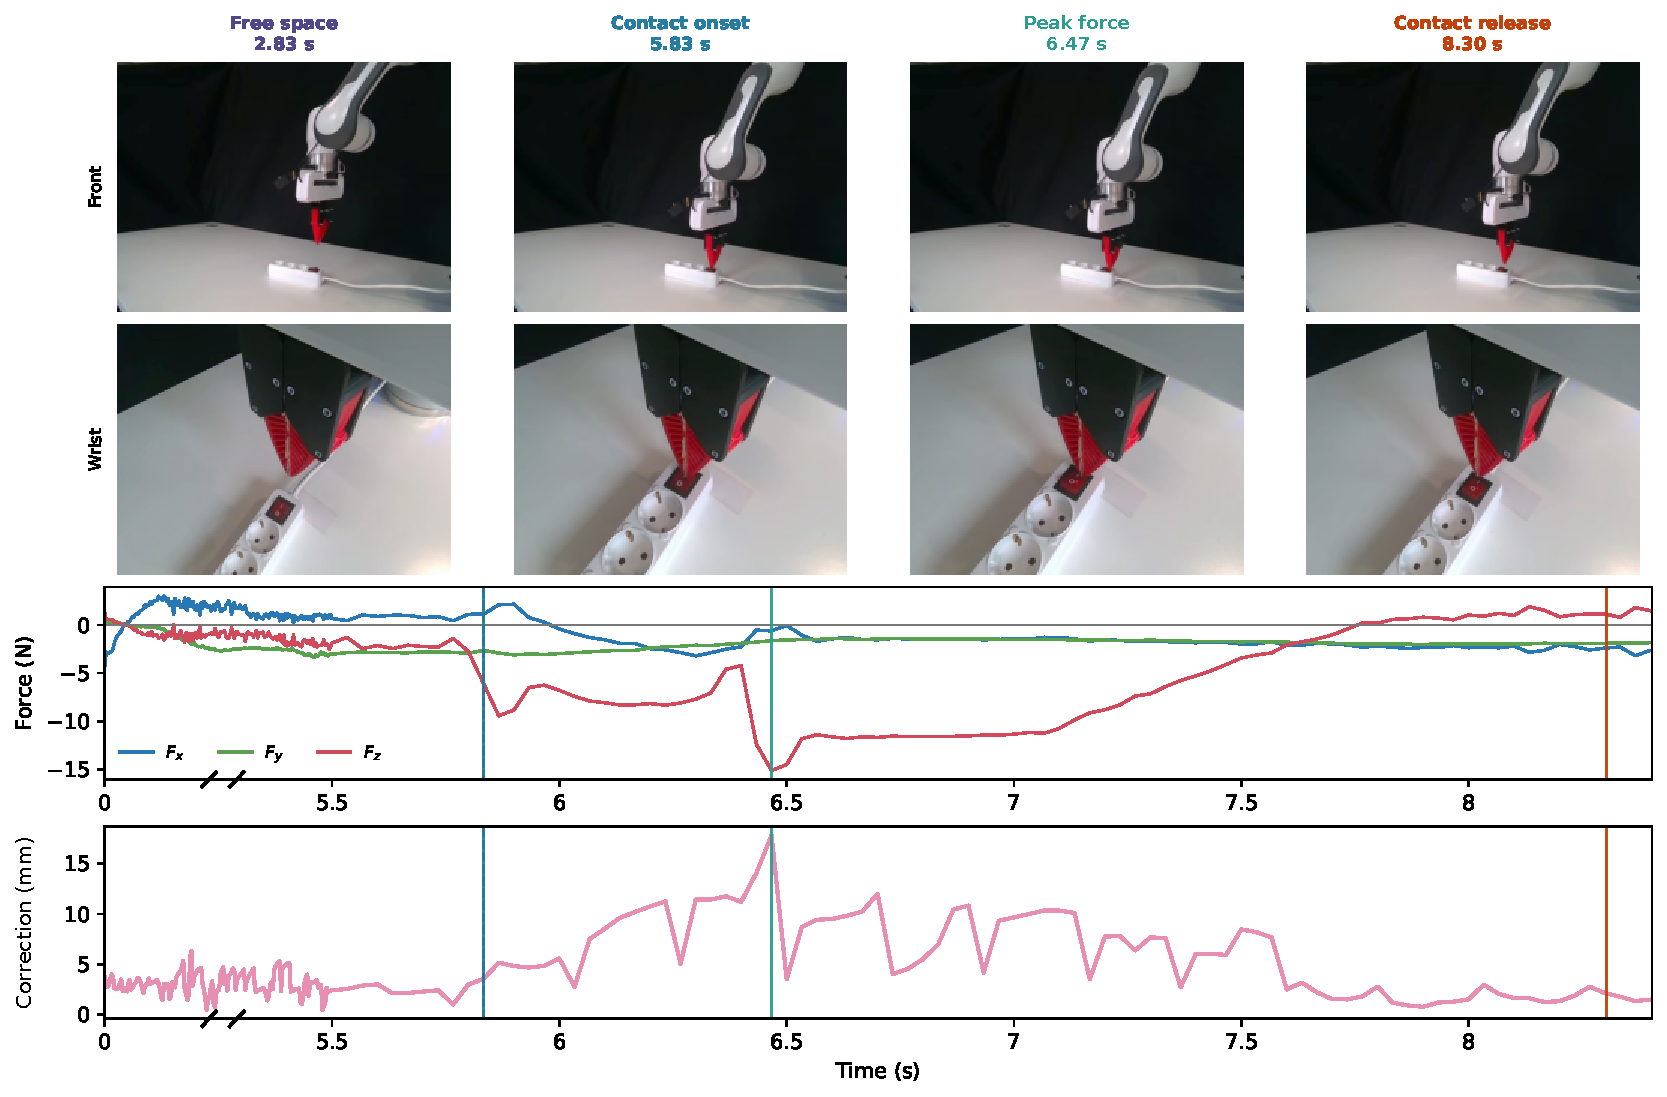
\includegraphics[width=\columnwidth]{figures/fig06_button_pressing_rollout.pdf}
    \caption{Representative rollout of Button Pressing. The observations show four interaction phases. The traces plot robot-estimated end-effector force components and translational correction magnitude over the contact interval; vertical lines mark the three displayed contact transitions, while the earlier free-space frame precedes the axis break.}
    \label{fig:qualitative_button}
\end{figure}

\subsection{Runtime and Reference-Action Delay}
\label{sec:exp_runtime}

We measure the forward-pass latencies of the reference-action and correction pathways and evaluate task performance under additional reference-action latency.

\noindent\textbf{Forward-pass latency.}
The correction forward pass takes $2.43$~ms, below the $10$-ms interval between robot command transmissions (Table~\ref{tab:runtime}). The Temporal Teacher and reference-action forward passes both exceed that interval. By reusing a reference action, the correction pathway avoids a new generative prediction at each query.

\begin{table}[t]
    \centering
    \scriptsize
    \setlength{\tabcolsep}{2pt}
    \caption{Forward-pass latency with batch size one under the Button Pressing deployment workload, reported as mean $\pm$ standard deviation over repeated passes on the deployment workstation.}
    \label{tab:runtime}
    \begin{tabular}{lc}
        \toprule
        \textbf{Method/path} & \textbf{Forward latency (ms)} $\downarrow$ \\
        \midrule
        ImplicitRDP & $12.86 \pm 0.23$ \\
        Temporal Teacher & $176.4 \pm 5.9$ \\
        ForceDelta reference action & $189.7 \pm 6.8$ \\
        ForceDelta correction & $\mathbf{2.43} \pm 0.12$ \\
        \bottomrule
    \end{tabular}
\end{table}

\noindent\textbf{Sensitivity to reference-action delay.}
We evaluate USB Insertion and Plug Insertion with $0$, $100$, and $200$~ms of additional reference-action latency, using $10$ trials per task, method, and delay. From $0$ to $200$~ms of additional delay, success decreases by $15$ percentage points for ForceDelta-VLA and $25$ points for the Temporal Teacher (Fig.~\ref{fig:latency_sensitivity}). Mean peak force over successful trials increases by $3.7$~N and $9.6$~N, respectively. These results support updating corrections between reference-action updates.

\begin{figure}[t]
    \centering
    \begin{minipage}[c]{0.49\columnwidth}
        \centering
        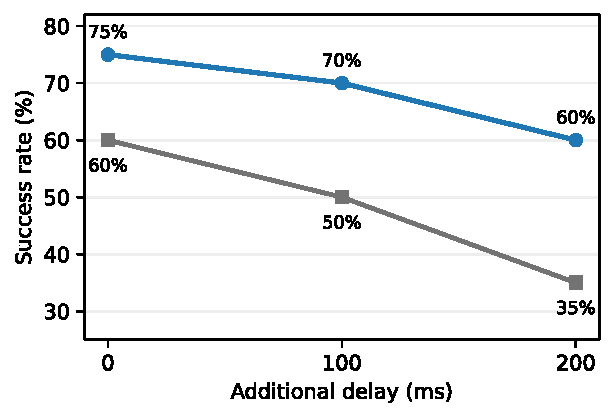
\includegraphics[width=\linewidth]{figures/fig07a_delay_success.pdf}
    \end{minipage}\hfill
    \begin{minipage}[c]{0.49\columnwidth}
        \centering
        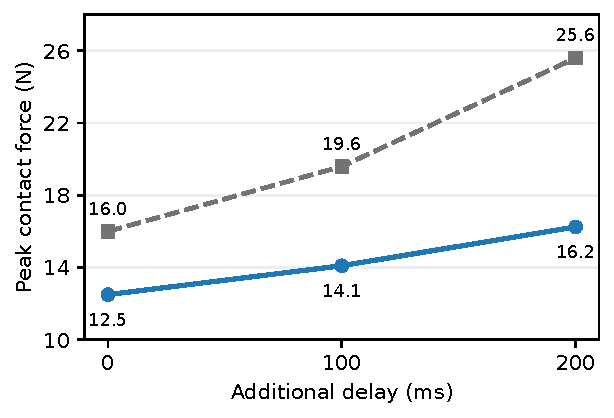
\includegraphics[width=\linewidth]{figures/fig07b_delay_peak_force.pdf}
    \end{minipage}
    \caption{Sensitivity to additional reference-action latency on the two insertion tasks. Left: success rate. Right: peak force over successful trials. Blue solid lines with circular markers denote ForceDelta-VLA; gray dashed lines with square markers denote Temporal Teacher.}
    \label{fig:latency_sensitivity}
\end{figure}

\subsection{Ablation Studies}
\label{sec:exp_ablation}

The ablations ask three questions: how the correction target should be defined, whether the fast policy should predict separate corrections, a combined correction, or complete actions, and how training should account for asynchronous execution (Table~\ref{tab:ablation}). All variants are evaluated on USB Insertion, single-arm Whiteboard Wiping, Plug Insertion, and Drawer Opening.

\noindent\textbf{Ablation setup.}
Execution ablations retain the trained model: \textbf{Reference action only} disables both corrections; \textbf{w/o force correction} disables the force output; \textbf{w/o learned delay correction} disables the full delay output, including reference-state alignment; and \textbf{Zeroed correction input} supplies an all-zero force history while retaining the force branch. The remaining variants retrain the affected policy. Their changes are described with the corresponding results below.

\begin{table}[t]
    \centering
    \scriptsize
    \setlength{\tabcolsep}{2pt}
    \caption{Ablations on four tasks, with 20 trials per task. Peak force: mean $\pm$ standard deviation over successful trials.}
    \label{tab:ablation}
    \begin{tabular}{lcccc}
        \toprule
        & \multicolumn{2}{c}{\textbf{Success rate} (\%) $\uparrow$}
        & \multicolumn{2}{c}{\textbf{Peak force} (N) $\downarrow$} \\
        \cmidrule(lr){2-3}\cmidrule(lr){4-5}
        \textbf{Variant} & \textbf{Single} & \textbf{Biman.}
        & \textbf{Single} & \textbf{Biman.} \\
        \midrule
        \multicolumn{5}{l}{\emph{Execution/component ablations}} \\
        Reference action only & $62.5$ & $50.0$ & $16.7 \pm 6.9$ & $18.2 \pm 7.6$ \\
        w/o force correction & $70.0$ & $57.5$ & $15.4 \pm 5.8$ & $17.1 \pm 6.3$ \\
        \shortstack[l]{w/o learned\\delay correction} & $77.5$ & $67.5$ & $13.2 \pm 4.1$ & $14.5 \pm 5.0$ \\
        Zeroed correction input & $65.0$ & $55.0$ & $15.9 \pm 6.4$ & $17.7 \pm 7.0$ \\
        \textbf{ForceDelta-VLA (full)} & $\mathbf{85.0}$ & $\mathbf{75.0}$ & $\mathbf{11.7} \pm 3.1$ & $\mathbf{12.8} \pm 3.8$ \\
        \midrule
        \multicolumn{5}{l}{\emph{Supervision/decomposition ablations}} \\
        \shortstack[l]{Demonstration-derived\\correction target} & $72.5$ & $57.5$ & $14.6 \pm 5.2$ & $16.5 \pm 6.1$ \\
        \shortstack[l]{Zero-wrench\\teacher query} & $65.0$ & $55.0$ & $16.1 \pm 6.7$ & $17.3 \pm 6.5$ \\
        w/o schedule replay & $77.5$ & $62.5$ & $13.8 \pm 4.7$ & $15.6 \pm 5.8$ \\
        \shortstack[l]{Single combined-\\correction head} & $75.0$ & $65.0$ & $13.5 \pm 4.3$ & $14.9 \pm 4.9$ \\
        \shortstack[l]{Fast full-action\\distillation} & $67.5$ & $52.5$ & $15.2 \pm 5.6$ & $17.9 \pm 7.4$ \\
        \textbf{ForceDelta-VLA (full)} & $\mathbf{85.0}$ & $\mathbf{75.0}$ & $\mathbf{11.7} \pm 3.1$ & $\mathbf{12.8} \pm 3.8$ \\
        \bottomrule
    \end{tabular}
\end{table}

\begin{samepage}
\noindent\textbf{How should correction supervision be defined?}
\textbf{Demonstration-derived correction target} replaces the force target with the demonstrated action minus the force-agnostic teacher prediction at the same query state. Success decreases by $12.5$ and $17.5$ percentage points on the single-arm and bimanual platforms, respectively. This comparison favors defining force supervision through teacher predictions matched in context, state, and sampling noise. \textbf{Zero-wrench teacher query}, used for both reference generation and target construction, also lowers success, supporting the learned force-agnostic mode.

\end{samepage}

\noindent\textbf{What should the fast policy predict?}
Removing the force correction reduces success by $15$ and $17.5$ percentage points and increases mean peak force over successful trials by $3.7$ and $4.3$~N on the single-arm and bimanual platforms, respectively. The force branch thus contributes to both task completion and contact-force reduction. Removing both corrections lowers success further. Zeroing the force history also performs worse than disabling the force output, indicating that the active branch depends on force feedback.

\textbf{Single combined-correction head} trains one head on the summed target and reduces success by $10$ percentage points on both platforms, favoring separate supervision and prediction of the two corrections. \textbf{Fast full-action distillation} of the teacher's pose actions also performs worse under the same compact student architecture, inputs, and update schedule. This favors reusing reference actions and assigning the student to predict their corrections.

\noindent\textbf{How does asynchronous adaptation contribute?}
Disabling the learned delay correction reduces success by $7.5$ percentage points on both platforms and increases peak force, supporting the adjustment for reference-action mismatch and reference-state alignment. Omitting \textbf{schedule replay} reduces success by $7.5$ and $12.5$ percentage points on the single-arm and bimanual platforms, respectively. The student therefore also benefits from training on delayed references.

\subsection{Generalization to Unseen Objects}
\label{sec:exp_physical_generalization}

We evaluate USB Insertion, Object Flipping, and bimanual Whiteboard Wiping with the unseen objects shown in Fig.~\ref{fig:physical_generalization_objects}.

\begin{table}[!htbp]
    \centering
    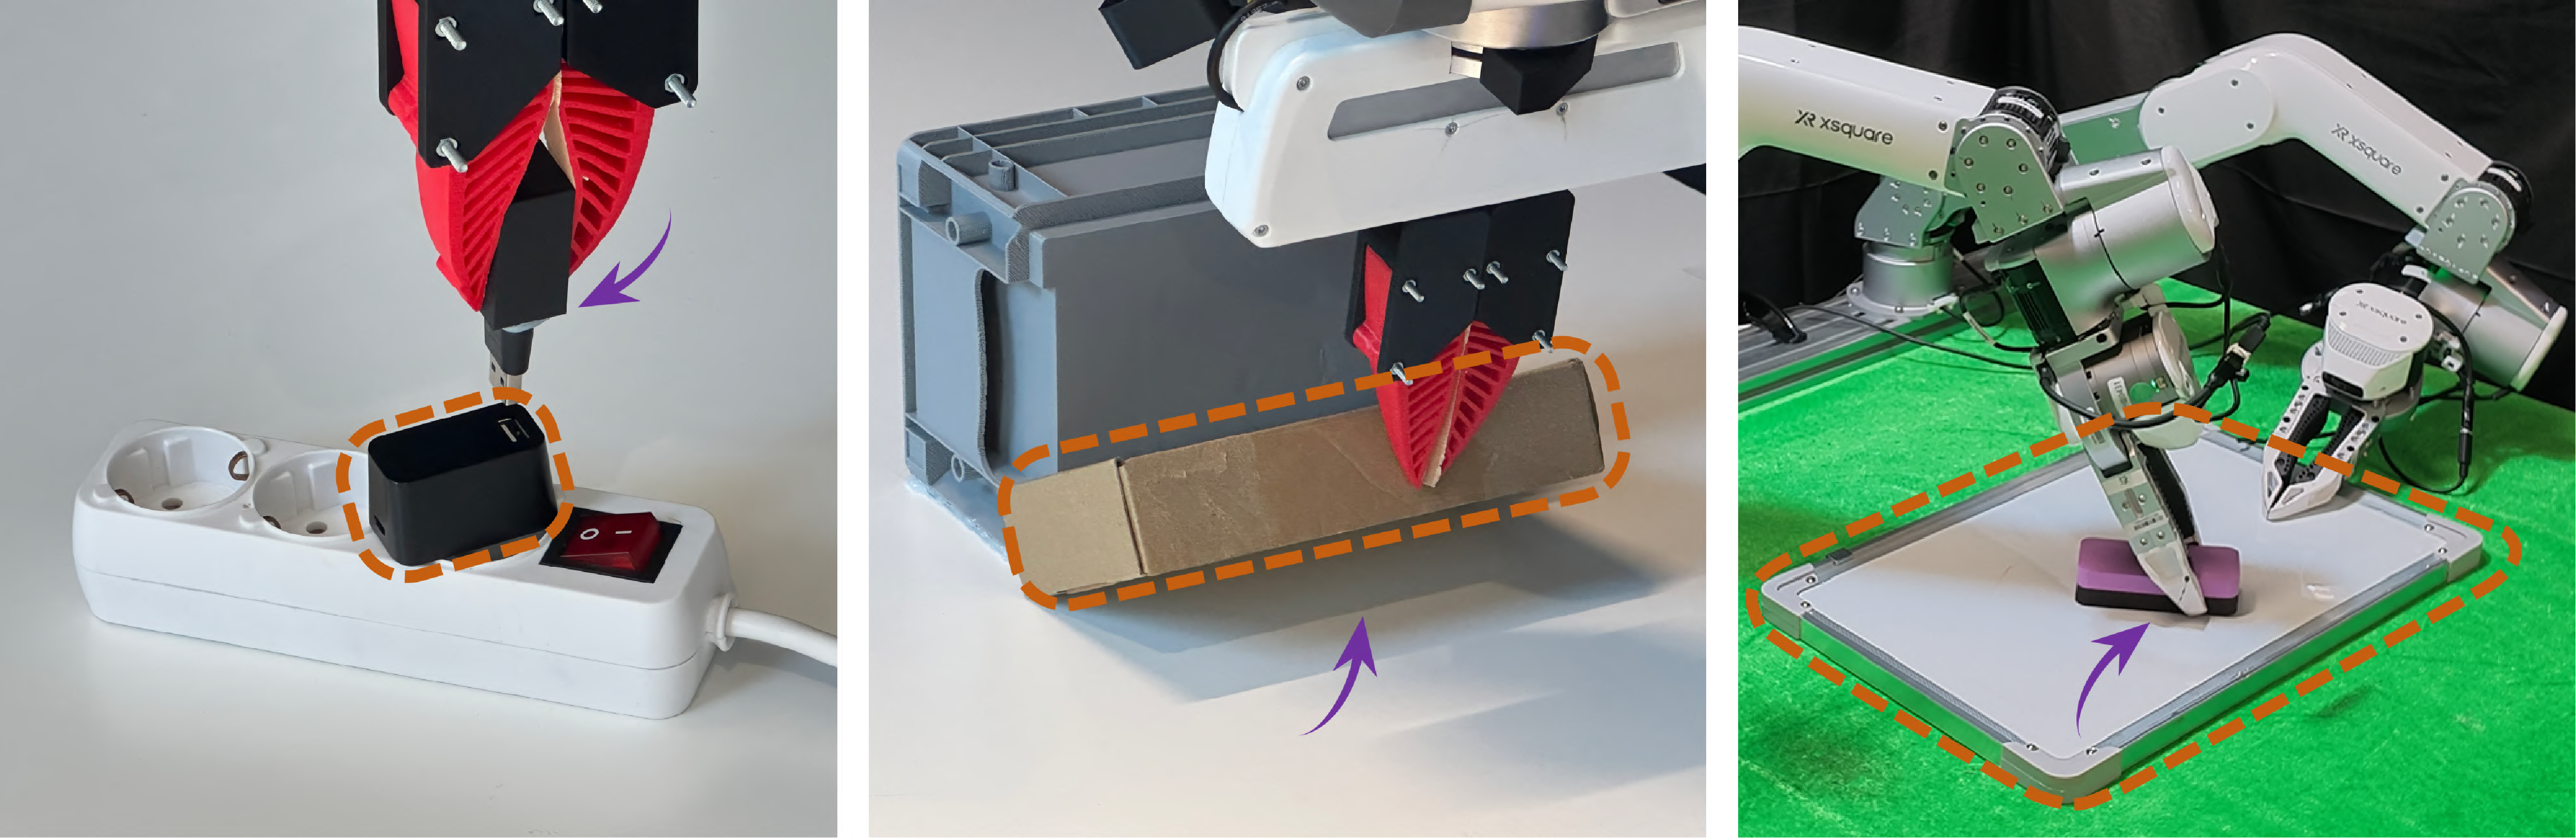
\includegraphics[width=0.85\columnwidth]{figures/fig08_unseen_objects.pdf}
    \begingroup
    \captionof{figure}{Generalization evaluation. From left to right: USB Insertion, Object Flipping, and bimanual Whiteboard Wiping.}
    \label{fig:physical_generalization_objects}
    \endgroup

    \scriptsize
    \setlength{\tabcolsep}{5pt}
    \caption{Generalization with unseen objects: 10 trials per task, 30 per method. Peak force: mean $\pm$ standard deviation over successful trials.}
    \label{tab:physical_generalization}
    \begin{tabular}{lcc}
        \toprule
        \textbf{Method} & \textbf{Success rate} (\%) $\uparrow$ & \textbf{Peak force} (N) $\downarrow$ \\
        \midrule
        ImplicitRDP & $16.7$ & $45.9 \pm 10.5$ \\
        Temporal Teacher & $40.0$ & $21.8 \pm 5.2$ \\
        \textbf{ForceDelta-VLA (Ours)} & $66.7$ & $13.6 \pm 3.7$ \\
        \bottomrule
    \end{tabular}
\end{table}

On unseen objects, ForceDelta-VLA improves success over the Temporal Teacher by $26.7$ percentage points and reduces mean peak force over successful trials by $8.2$~N (Table~\ref{tab:physical_generalization}). The new USB port is particularly challenging for the Temporal Teacher. For ImplicitRDP, failures often occur while establishing contact: the policy misses the replacement eraser during grasping or fails to initiate the downward insertion motion.

\subsection{Failure Analysis}
\label{sec:exp_limitations}

In failed USB and plug insertion trials, the robot often reached the target region but contacted the rim or entered with a small orientation error. Once the connector jammed, the reference action often continued advancing, and the corrected motion did not retreat far enough to clear the jam and retry.

In cabinet and drawer opening, pulling sometimes began before stable contact with the handle was established. Recovery required releasing contact, repositioning the gripper, or approaching again. Wiping and object-flipping failures involved contact on an unintended side or loss of the intended contact geometry, requiring a different approach direction.

Reference-update delay further reduced insertion success (Fig.~\ref{fig:latency_sensitivity}). During this delay, the robot could enter a new contact state while the student continued correcting a chunk generated before that change. These failures point to the need for reference updates that initiate retreat, reestablish contact, or change the approach direction.
